\chapter{Fejlesztői dokumentáció}
\label{ch:impl}

\section{Webalkalmazás specifikáció}
Az alkalmazás fő célja egy olyan működő webáruház bemutatása, ami \citeauthor{MEAN} (MongoDB, Express.js, Angular, és Node.js - solution stack) nevezetű szoftverköteg segítségével készült. A \citeauthor{MEAN}  megoldásverem egy ingyenes nyílt forráskódú szoftverek halmaza, ami lehetőséget kínál dinamikus weboldalak készítésére. A webalkalmazás két főrészre osztható kliensoldali és szerveroldali (idegen nyelven: front-end és back-end) részre. A kliensoldal leglényegesebb feladata, hogy a felhasználó által is látott weboldalt megjelenítse grafikai UI/UX(rövidítés feloldása: User interface/User experience)dizájn implementálásával. Nevezetesen egy olyan rendszer, ami képes a felhasználó számára felületet és élményt biztosítani. Miközben a szerveroldal elsődleges feladata az alkalmazás úgynevezett business logikájának a megvalósítása. Ezen felül képes az adatok feldolgozására és hitelesítésére is. A következő ábrán szeretném reprezentálni milyen módon épül fel a webalkalmazás, továbbá megismertetni a két oldal kommunikációs kapcsolatát.

\begin{figure}[H]
	\centering
	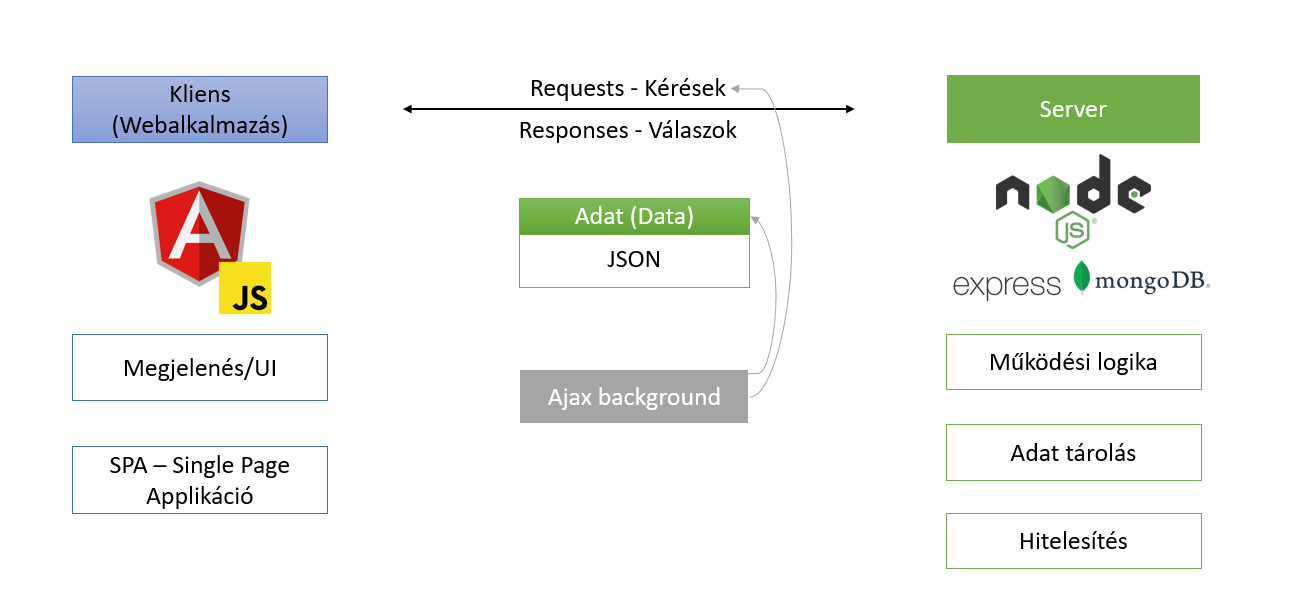
\includegraphics[width=1.0\textwidth,height=250px]{images/alkalmazas_bemutatasa.png}
	\caption{Az alkalmazás bemutatása}
	\label{fig.picture-1}
\end{figure}

A \ref{fig.picture-1}-es ábrán látható a két oldal miképpen osztja meg az információkat egymás között. A front-end pontosabban mondva a kliensoldal \citeauthor{Angular} keretrendszerben \citeauthor{TypeScript} segítségével íródott. A front-end kommunikációja úgynevezett requestekkel más néven kérésekkel (json típusú adattovábbítással) a háttérben aszinkron módon történik amire a szerveroldal responsokkal egyszóval válaszokkal felel. A back-end \citeauthor{Node.js} szoftverrendszer alapú, ami \citeauthor{Express} segítségével íródott. Az adatok tárolásáért a \citeauthor{MongoDB} nevezetű adatbázis felel.

\bigskip
A következő blokkokban szeretném tételesen demonstrálni a fentebb említett front-end és back-end oldalakon használt módszerek alkalmazását és működését. Ezen felül szándékomban áll ismertetni az általam alkalmazott szoftverek technikai tulajdonságaikat.

\section{Kliensoldalon használt technológiák bemutatása}
A dokumentáció és az egész program fő eleme az Angular keretrendszer használata, aminek a segítségével dinamikus webalkalmazások hozhatóak létre. Az Angular egy nyílt forráskódú a Google által fejlesztett JavaScript nyelven írt front-end keretrendszer. Ebben a fejezetben szeretném kellőképpen kifejteni miért ezt a rendszert választottam az alkalmazás megírásához ezen felül alaposabban bemutatni a működését és főbb tulajdonságait a \ref{fig.picture-2}-es ábra segítségével. 

\subsection{Angular keretrendszer}

\begin{figure}[H]
	\centering
	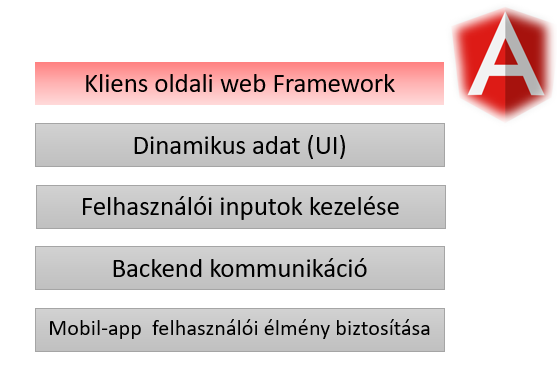
\includegraphics[width=1.0\textwidth,height=250px]{images/angular_bemutatas.png}
	\caption{Az Angular keretrendszer bemutatása}
	\label{fig.picture-2}
\end{figure}

 Az Angular egyik legfőbb tulajdonsága, hogy egy kliensoldali keretrendszerről beszélhetünk az esetében. Ennek köszönhetően képes feldolgozni és megjeleníteni a back-end felől érkező adatokat, így egy dinamikus webalkalmazást kapunk. Ezt úgy tudja biztosítani, hogy képes kapcsolatot kialakítani a szerveroldallal. Továbbá lehetőséget nyújt a felhasználó által beérkezett adatokat fogadására és kezelésére, ezen funkciója segítségével egy modern UI/UX felület készítésére alkalmazhatjuk. A program megírása során a 13.0.4 legújabb verziójú Angular CLI-t telepítettem. Minden ezen jellemzői hozzátesznek, ahhoz, hogy Single Page Applikációnak(továbbiakban: SPA) nevezzük az általa támogatott weboldalakat. Olyan webhelyeket hívhatunk SPA-nak, amelyek egyetlen oldalra tölti be dinamikusan az adatokat, más szóval minden eleme egy oldalon található. Ennek köszönhetően a weboldalon való navigáláshoz nem kell betölteni külön DOM vagyis Dokumentumobjektum-modelleket.

\section{Kliensoldal működése}
A weboldal felépítéséért, megjelenéséért és kinézetéért a HTML, TypeScript és SCSS hármas programozási nyelv felel. A HTML feladata az alkalmazás tartalmi megjelenítése, a scss pedig ezen tartalom formázása. A TypeScript pedig biztosítja a felhasználó által kiadott utasítások végrehajtását. Az Angular keretrendszerben ez a három nyelv egy-egy komponens darabjai.

\subsection{Komponensek}
A komponensek a programkód logikai darabjai. Két fő eleme van. Az első ilyen elem a templat-ek, ami az alkalmazás megjelenítéséért felel, ez tartalmazza a HTML-t. A második elem az osztályok amiben szerepelnek a metódusok és tulajdonságok, ez a rész a TypeScript fájlokban van definiálva.

\subsection{Modulok}
Az Angular alkalmazások modulárisak és saját moduláris rendszerrel rendelkezik, amit NgModules-nak nevezünk. Ennek a modulnak a segítségével különböző komponenseket, direktívákat és service fájlokat csoportosíthatunk a metaadatai segítségével. Az NgModule-nak öt ilyen metaadata van, aminek a használatával kategorizálhatjuk a komponenseinket felhasználás szerint.

NgModule metadatai:

\begin{itemize}
	\item deklarációk (declarations): az itt szereplő komponensek kifejezetten ahhoz a module-hoz tartoznak, ahol létrehoztuk őket
	\item exportok (exports): a deklarációban használt komponensek azon részhalmaza, amiknek láthatónak kell lennie máshol létrehozott komponensek számára
	\item importok (imports): olyan modulokat tartalmaz amiket a deklarációnál implementált komponensek használnak
	\item szolgáltatók (providers): olyan osztályok szerepelnek itt, amelyek létrehozzák és menedzselik a service objektumokat első alkalomkor, amikor az Angularnak szüksége van a függőségek feloldásához.
\end{itemize}

\subsection{Interfészek}
Az interfészek olyan specifikáció az angular frameworkben, amelyek egy osztály által megvalósítandó tulajdonságok és metódusok összefüggő halmazát határozza meg. Tehát a segítségével létrehozható pár alapvető szabály a tulajdonságokra és a metódusokra amiket használunk az osztályon belül.

\subsection{Service fájlok}
A projektben a servise fájlok tartalmazzák azokat a függvényeket, amiknek a segítségével kapcsolatot alakíthatunk ki a szerveroldallal. Ezek a fájlok tartalmaznak bizonyos request kéréseket, amiknek a segítségével a felhasználó elindíthatja az adatlekérés folyamatát. A függvények kigyűjtésének célja, hogy egyszerűbben elérhetőek legyenek több komponens számára.

\subsection{Admin mappa}
Ez a mappa tartalmazza az adminisztrációs oldal megjelenítéséhez szükséges fájlokat elkülönítve a többi komponenstől. Úgy gondolom erre azért volt szükség, mert a két oldal szerkezeti felépítése eltérőek egymástól, továbbá segítette a fejlesztés során ezeket elszeparálva tartani.

\subsection{Pages mappa}
A webalkalmazás összes olyan komponense található ebben a mappában, ami nem kapcsolódik hitelesítési funkció az eléréséhez. Az áruház öt fő oldala található meg itt.

\begin{compactitem}
	\item Főoldal/Kezdőlap: összefoglalja a hírek és a termékek oldalát
	\item Hírek: az oldal üzemeltető által megosztott fontosabb információk
	\item Termékek: minden olyan termék, amit eladásra szánnak
	\item Rólunk: az oldal üzemeltetőjével kapcsolatos információk - kapcsolattartás
	\item Bevásárlókosár:  a felhasználó által kiválasztott termékek
\end{compactitem}

\subsection{Oldalak közötti navigáció}
Az oldalak közötti koordinálást az előbbiekben kifejtett modul fájlok egyike kezeli. Angularban a legjobb mód az, hogy ha a routerbe betöltést és a konfigurálást különállóan történik. A konfigurálás az AppRoutingModuleban zajlik, míg a betöltés a legfelső szintű module azaz az AppModuleban van importálva, ami útválasztóként is szolgál.

\subsection{Shared mappa}
A shared mappa tartalmazza azokat a komponenseket és angular kiegészítő csomagokat, amiket több oldalon is megjelenítésre kerülnek. Ezek a komponensek és packegek a következők:

\begin{description}
	\item[Angular Material] egy felhasználói felület (UI) komponens könyvtár. Segítségével gyorsítja a fejlesztési folyamatot, konzisztens és elegán felületet biztosítva.
	\item[Alert üzenetek] segítségével a felhasználó által elindított folyamatok állapotáról nyújthatunk információt.
	\item[Nyelvválasztás] lehetőséget biztosít az oldalon található adatok többnyelvű megjelenítését.
	\item[Vissza gomb és a go to top gomb] a nevéből kiindulva olyan gombok amiknek lehetőségével egyszerűbb használatot biztosít a felhasználók számára.
	\item[Chatbot] animációval rendelkező beszélgetési felület, ami lehetőséget nyújt arra, hogy a felhasználó gyors információt szerezzen az adott szolgáltatásokkal kapcsolatban. A chatbot részletes bemutatása a 3.7-es fejezet Forráskódok 3.7.1-es Kliensoldali forráskódok alfejezetében található,
\end{description}

\subsection{Egyéb fájlok és mappák}
Ebben a blokkban szerepel minden olyan mappa és fájl amit nem tudtam az előző fejezetekhez kapcsolni funkciójuk különbségük miatt.

\begin{itemize}
	\item Assets mappa: minden olyan képfájlt tartalmaz, amit nem dinamikusan kapunk a szervertől. Ilyen képek például az oldalon használt logók, vagy borítóképek.
	\item Enviroments mappa: az ebben szereplő fájlok tartalmazzák a szerveroldal eléréséhez szükséges url címet.
	\item Theme mappa: olyan stílusfájl, ami a komponensekben használt színek gyűjteményét tartalmazza.
	\item style.scss: minden olyan stílus elem leírása amit a komponensek közösen használnak
\end{itemize}

\section{Szerveroldalon használt technológiák bemutatása}
A szerveroldalon használt (3.1-es blokkban már említésre kerülő) módszerek kiválasztásuk előtt kulcsfontosságú szempontjuknak tartottam, hogy az Angular keretrendszerhez megfelelő kompatibilitással rendelkezzenek és alkalmazni tudjam őket a szakdolgozat elkészítése során. A következő technológiák mind olyan szoftverek, frameworkök vagy szerverek amikhez számtalan monográfia elérhető az interneten, ezzel támogatva a későbbiekben létrehozott projekteket. A következő felsorolásban összefoglalásképpen összegyűjtöttem az alkalmazásban fellelhető általam használt szoftvereket és verziószámukat:

\begin{compactitem}
	\item Node.js: 14.15.4
	\item Express.js: 4.17.1
	\item Mongoose: 6.0.12
	\item MongoDB Atlas
\end{compactitem}

\bigskip
A fejezet további részében szeretném ismertetni a fentebb felsorolt technológiák jellegzetes tulajdonságaikat, főbb jellemzőiket további ábrák segítségével.

\subsection{Node.js szoftverrendszer}

\begin{figure}[H]
	\centering
	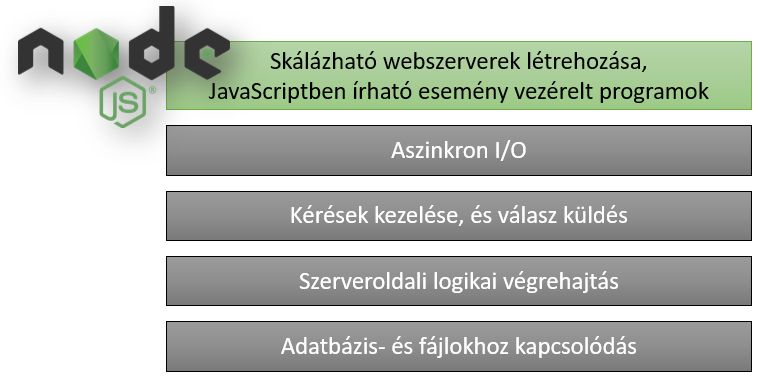
\includegraphics[width=1.0\textwidth,height=220px]{images/nodejs_bemutatasa.png}
	\caption{NodeJS bemutatása}
	\label{fig.picture-3}
\end{figure}

A webáruház back-end megírásánál 14.15.4-es verziójú Node.js szoftverrendszert használtam. A \ref{fig.picture-3}-as ábrán látható a Node.js bemutatása, ami összefoglalja a szoftverrendszer fontosabb jellemzőit. Az illusztráció első dobozában olvasható miszerint a Node.js skálázható webszerverek létrehozására alkalmas más szóval egy olyan rendszert tudunk létrehozni a támogatásával, ami több felhasználót képes egyidejűleg kiszolgálni. Ezenfelül JavaScript nyelv segítségével olyan programok írhatóak, amely a komponensek közötti esemény interakciókat tekinti alapul, mászóval eseményvezérelt programok megírására alkalmas (ilyen például egy egérkattintás vagy billentyű leütés). Folytatólag a Node.js aszinkron tulajdonságával lehetővé teszi, hogy a kliensoldalról érkező kérések várakozási sorrendbe kerüljenek, ennek következtében a kliensoldal tovább folytathatja a feladatát. 

\subsection{Express.js framework és Mongoose programozási könyvtár}

\begin{figure}[H]
	\centering
	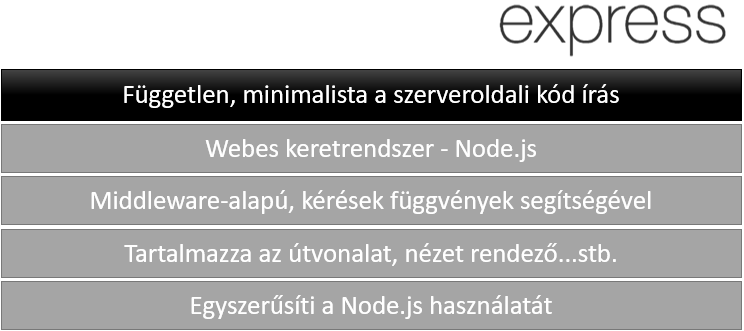
\includegraphics[width=0.8\textwidth,height=220px]{images/express_bemutatasa.png}
	\caption{Express bemutatása}
	\label{fig.picture-4}
\end{figure}

A szerveroldal áttekinthetőbb és olvashatóbb kódírása érdekében a webáruház fejlesztése során az Express.js 4.17.1-es verzióját használtam. Az Express egy webes keretrendszer a Node.js nehézség nélküli használatára lett fejlesztve. A \ref{fig.picture-4}-es ábrán látható az Express attribútumainak ismertetése. Az illusztráción felvetettem, hogy az Express egy Middleware-típusú rendszer következésképpen lehetővé teszi a MongoDB adatbázis szoftverhez való zavartalan kapcsolódást a Mongoose 6.0.12 verziójával kiegészítve, ami egy JavaScript-ben írt objektum-orientált programozási könyvtár.

\subsection{MongoDB adatbázisszerver}

\begin{figure}[H]
	\centering
	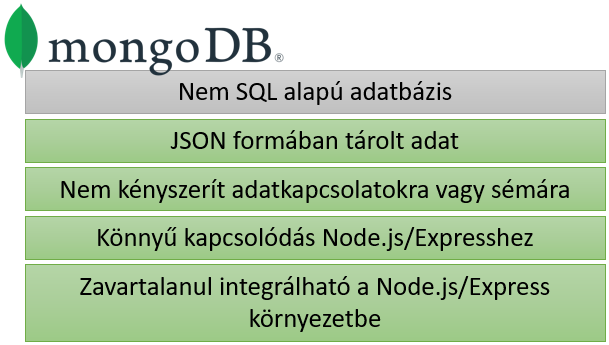
\includegraphics[width=0.8\textwidth,height=220px]{images/mongodb_bemutatasa.png}
	\caption{MongoDB bemutatása}
	\label{fig.picture-5}
\end{figure}

A MongoDB egy nyílt forráskódú, NoSQL adatbázisszerverek közé sorolt szoftver. A NoSQL magyarán Nem SQL típusú adatbázisrendszert jelent. Jellemzően nem rekordokat és táblázatokat tárolnak mint az SQL típusú szerverek, hanem független dokumentumokat és gyűjteményeket archiválnak. Személyes véleményem szerint a \ref{fig.picture-5}-ös illusztrációval alátámasztva egyik legfőbb pozitív tulajdonságának éreztem a alkalmazás írása során, hogy az adatok JSON formátumban képes tárolni. Következésképpen a request és response folyamatok egyszerűsített és gyors működését képes biztosítani, mindeközben lehetővé teszi a kliensoldalon megjelenítendő információk könnyebb feldolgozását. 
\bigskip

\subsection{NoSQL vs SQL adatbázisok összehasonlítása}

A következő grafikai ábrán szándékozom röviden bemutatni és összehasonlítani a Nem SQL és az SQL alapú adatbázisokat jellegzetes tulajdonságaik szerint.

\begin{figure}[H]
	\centering
	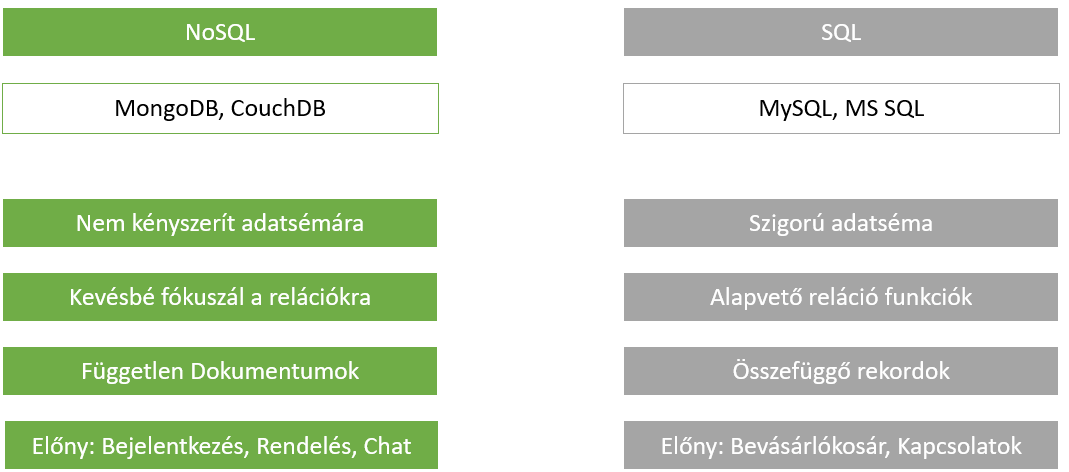
\includegraphics[width=1.0\textwidth,height=220px]{images/nosql_bemutatasa.png}
	\caption{NoSQL vs SQL adatbázisok összehasonlítása}
	\label{fig.picture-6}
\end{figure}

Mint a \ref{fig.picture-6}-os ábrán megfigyelhető szempontok szerint egy webáruházban kezelt adatok tárolására a No SQL adatbázisok is kifejezetten alkalmasok. A NoSQL adatbázisszerverek jellemző tulajdonságai kulcsfontosságú szempontokkal szolgált a webáruház adatbázisának kiválasztásánál.

\section{Szerveroldal működése}

Ebben a fejezetben részletesen prezentálom az alkalmazás szerveroldali működését példának okáért milyen request és response hívások találhatóak a kódban, hogyan létesít kapcsolatot a webalkalmazás az adatbázissal...stb., valamint külön kitérek az adminisztrációs oldalon található hitelesítésére alkalmazott technikára is.

\subsection{RESTful API - Végpont tervek bemutatása}

A webáruház megírása során RESTful API-t (feloldva: Representational State Transfer Application programming interface) magyarán reprezentáción alapuló állapotátvitel nevezetű architekturális módszert használtam. Az API-k segítségével a felhasználó számára elérhető a weboldalon számos interakció. Ilyen interakciónak számít például a bejelentkező felület.

\bigskip
Az alábbi illusztráción szeretném bemutatni az alkalmazásban használt REST API hívásokat, ennek okán a \ref{fig.picture-7}-es ábrán láthatók a programban megírt végpontok.


\begin{figure}[H]
	\centering
	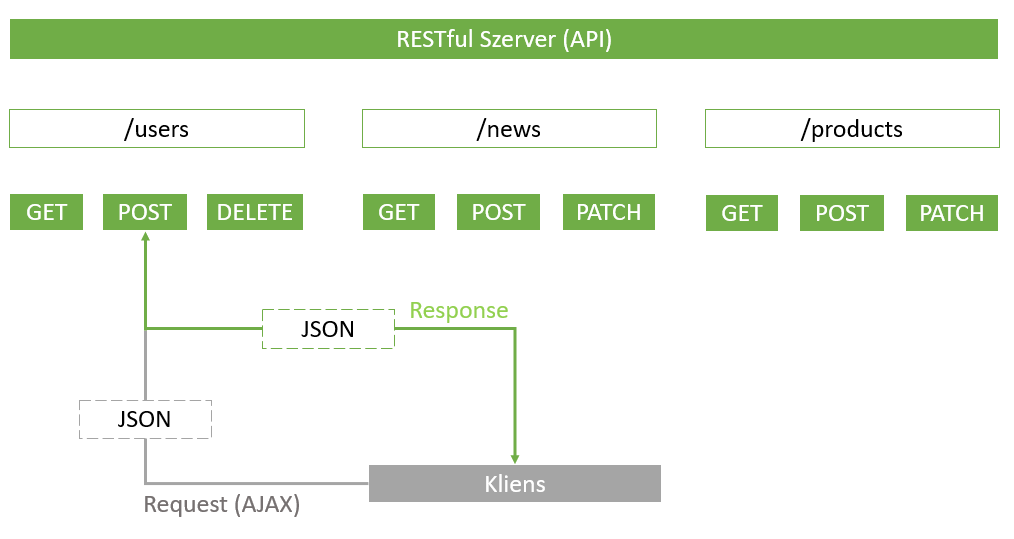
\includegraphics[width=1.0\textwidth,height=220px]{images/restapi_bemutatasa.png}
	\caption{Adatkezelés}
	\label{fig.picture-7}
\end{figure}

 A grafikán megfigyelhető hét különböző végpont ami az auth, hírek, termékek, termékcsoportok, üzenetek, chatek és rendeléseket fejezi ki. Az illusztrációt figyelemmel kísérve identifikálható, hogy nem minden végpont rendelkezik ugyan azokkal a kérésekkel. Szemléltetésképp vegyük figyelembe a hírekhez vonatkozó responsokat amik a GET, POST, PATCH és DELETE függvények, ezzel szemben a auth-hoz kizárólag POST függvény tartozik. Ennek kifejezetten egy oka van, mégpedig az, hogy a webáruház egyes adatait nem szükséges módosítani tudni kliens oldalról.

\bigskip
A REST API-t megismerve és ezt az információt felhasználva szemléltethető és az alább ábrán látható miképpen éri el a felhasználó által kezdeményezett kérés az adatbázist és hogyan kerül válaszra.

\begin{figure}[H]
	\centering
	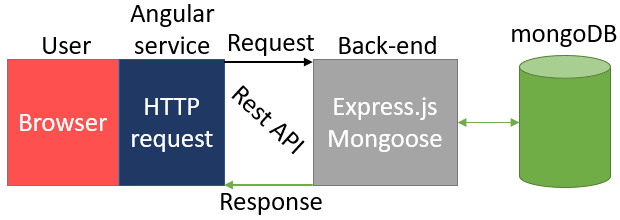
\includegraphics[width=1.0\textwidth,height=220px]{images/kapcsolat_szerver_bemutatas.png}
	\caption{Kapcsolat a szerverrel}
	\label{fig.picture-8}
\end{figure}

A fenti \ref{fig.picture-8}-as ábrával és az alább található alkalmazásban szereplő kódsorok segítségével szeretném bemutatni, hogy a felhasználó által indított kérés milyen sorrendben jut el az adatbázishoz és miképpen tér vissza hozzá.

\bigskip
Felhasználó interakcióba lép a felülettel (például: egy gombra kattintva~\ref{src:html}-es forráskód), ennek következményeként meghívódik egy a gombhoz tartozó TypeScript nyelven írt függvény \ref{src:ts}-es forráskód.

\lstset{caption={Felhasználói interakció - HTML fájl}, label=src:html}
\begin{lstlisting}[language=html]
	<form style="margin-top: 2rem;" [formGroup]="form" (submit)="onAddMessage()" *ngIf="!isLoading">
	....
	<button class="btn-secondary" type="submit" [disabled]="!confirmed.checked">
		{{'GENERIC.ACTION.SEND' | translate}}
	</button>
\end{lstlisting}

\lstset{caption={Interakció függvényhívás - TypeScript fájl}, label=src:ts}
\begin{lstlisting}[language=JavaScript]
	onAddMessage(): void {
		if(this.form.invalid) {
			this.alertService.warn('ALERT.WARN.INVALID_FORM');
			this.form.markAllAsTouched();
			this.isLoading = false;
			return;
		}
		this.isLoading = true;
		this.contactService.sendMessage(
			this.form.value.firstName,
			this.form.value.lastName,
			this.form.value.email,
			this.form.value.description,
			this.form.value.image,
		)
		this.isLoading = false
		this.form.reset();
	}
\end{lstlisting}

Az előbb említett \ref{src:ts}-es forráskódban szereplő függvény átadja az adatokat a kliensoldalon található Service fájl sendMessage() nevezetű függvényének. Ez a fájl tartalmazza a következő \ref{src:service}-as forráskódban szereplő kódsort.

\lstset{caption={HttpClient POST request - Service TypeScript fájl}, label=src:service}
\begin{lstlisting}[language=JavaScript]
	sendMessage(
		firstName: string, 
		lastName: string, 
		email: string, 
		description: string, 
		image: File | string
	){
		const messagesData = new FormData();
		messagesData.append("firstName", firstName);
		messagesData.append("lastName", lastName);
		messagesData.append("email", email);
		messagesData.append("description", description);
		messagesData.append("image", image, firstName);
		this.http.post<{message: string, messages: Messages}>
		(environment.apiUrl + "messages", messagesData)
			.subscribe(responseData => {
				const messages: Messages = {
					id: responseData.messages.id,
					firstName: firstName,
					lastName: lastName,
					email: email,
					description: description,
					imagePath: responseData.messages.imagePath,
				};
				this.messages.push(messages);
				this.msgUpdate.next([...this.messages]);
				this.alert.success('ALERT.SUCCESS.ADD');
				this.router.navigate(["/contact"]);
			}, error => {
				this.alert.error(error.error.message);
			});
	}
\end{lstlisting}

Ebben a kódrészletben látható, ahogyan a kliens oldal HttpClient Angular package POST request segítségével a megadott útvonalon küld egy REST API kérést a szerveroldal felé.

\bigskip
A szerveroldal fogadja ezt a kérést és továbbítja a MongoDB felé. Az alábbi \ref{src:express}-es forráskódban Express - JavaScript nyelv segítségével megírt kódrészletben ez szerepel.

\lstset{caption={Express POST végpont - JavaScript}, label=src:express}
\begin{lstlisting}[language=JavaScript]
	exports.postMessages = (req, res, next) => {
		const url = req.protocol + "://" + req.get("host");
		const msg = new Messages({
			firstName: req.body.firstName,
			lastName: req.body.lastName,
			email: req.body.email,
			description: req.body.description,
			imagePath: url + "/images/messages/" + req.file.filename,
		});
		msg.save().then(result => {
			res.status(201).json({
				message: "Message added successfully",
				messages: {
					...result,
					id: result._id
				}
			});
		});
	}
\end{lstlisting}

Kliensoldalon és Szerveroldalon egyaránt látható a felhasználó által elindított kérés státuszát tartalmazó információ. A front-end-en egy úgynevezett AlertService componens segítségével kap visszaigazolást az elindított kérés befejezéséről, míg a back-end-en az adatbázis felé elküldött kérés kódrészletében található ez az információ.

\bigskip
A webalkalmazásban szereplő további REST API hívásokat tartalmazó példakódsorokat a 3.7-es Forráskódok 3.7.2-es Szerveroldali forráskódok nevezetű alfejezetben találhatóak.

\subsection{Hitelesítés - Adminisztrációs felület védelme}
Az alkalmazás megírása során akaratlagosan egy olyan webáruház létrehozása volt a végcélom, ami időszerű adatok kezelését tudja biztosítani. Következésképpen egy olyan felület megvalósítása gyakorlatban is, amely nem igényel programozón keresztüli beavatkozást. Ennek okán a szakdolgozat tartalmaz egy adminisztrációs oldalt, amely biztosítja a webalkalmazásban dinamikusan megjelenő adatok aktualitását, továbbá a leadott rendelések vásárlók által elküldött üzenetek megjelenítésére is szolgál. Kifejezetten ennek a blokk védelmében került bele külön hitelesítési felület.

\bigskip
Az alább található \ref{fig.picture-9}-es grafikán ez az engedélyezési folyamat elméleti működése látható.
 
\begin{figure}[H]
	\centering
	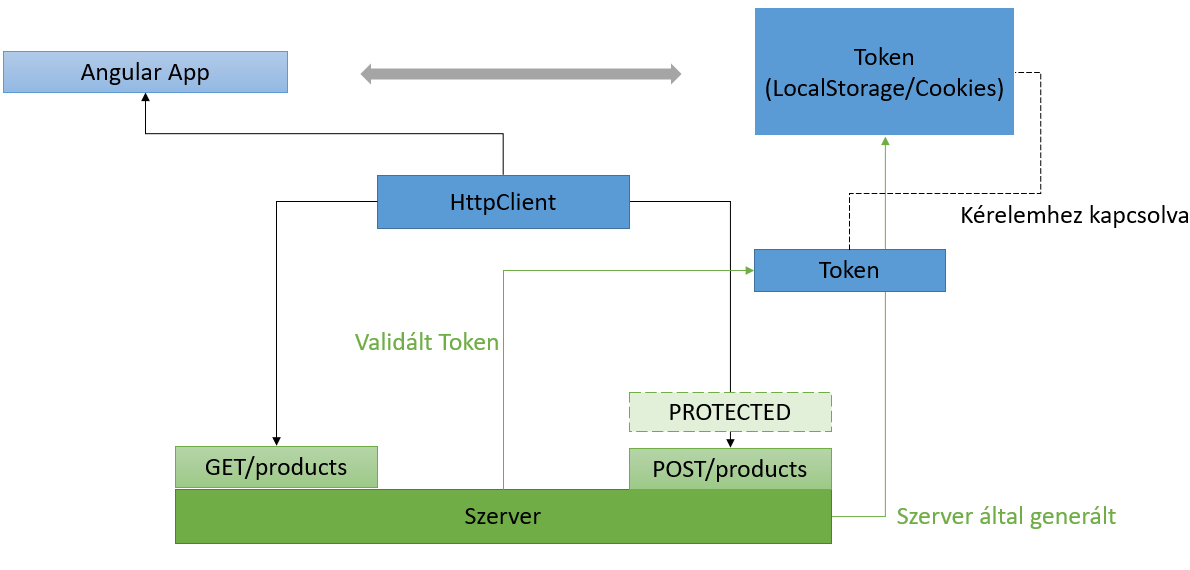
\includegraphics[width=1.0\textwidth,height=220px]{images/hitelesites_bemutatasa.png}
	\caption{Hitelesítés}
	\label{fig.picture-9}
\end{figure}

Az illusztráción ábrázolt hitelesítési folyamat a következőképpen történik. Az alkalmazás front-end-ről érkező GET/products kérésre engedélyezés nélkül kap választ a szervertől, mivel a webáruházban bejelentkezés hiányában is hozzáférhetővé kell tenni ezt az információt. Ezzel szemben a POST/products kérés nem következhet be hitelesítés nélkül. Tehát bejelentkezés során a szerver generál egy úgynevezett tokent és LocalStorage-ba elmenti, amit az új termék hozzáadás kérésnél ellenőriz. Az alkalmazásban ez a hitelesítési funkciót következőképpen valósul meg:

Ennek a funkciónak létrehozásánál két kiegészítő package-et úgynevezett bcryptjs-t és jsonwebtoken-t használja a programkód. Az előbbi lehetőséget nyújt bizonyos adatok titkosítására (ilyen adat például a belépési jelszó), az utóbbi pedig bizonyos REST API kérések érvényesítésére alkalmas. Mikor létrehozásra kerül egy új felhasználó a bcrypt package egy úgynevezett hash metódusát hívja meg a program, aminek segítéségével az új felhasználó jelszava titkosítva kerül be az adatbázisba. Ennek oka az, hogy ha véletlenül sikerül egy idegennek belépnie az adatbázisba, akkor ne tudja megszerezni az adott felhasználók jelszavát. Viszont, ha titkosítva kerül be az adat, a későbbiekben belépésnél nem lehet ellenőrizni, hogy a megfelelő jelszó került-e beírásra. Erre a problémára szolgál megoldásképp a bcryptjs compare metódusának használata, aminek segítségével összehasonlításra kerül az adott felhasználó adatbázisban szereplő jelszava és a begépelt jelszó hashelt változata, mivel ha pont a megfelelő adat kerül beírásra akkor a titkosított információnak megegyezőnek kell lennie az adatbázisban található jelszóval. Sikeres bejelentkezésnél a szerveroldal generál egy tokent a jsonwebtoken package segítségével és minden olyan kérésnél amihez szükséges autentikáció, ellenőrzésre kerül ennek az érvényes tokennek a létezése. A programkódban generált tokenek hitelessége egy óráig él.

Mindent összevetve az adminisztrációs felület védve van az illetéktelen felhasználók belépésétől és bizonyos funkciók végrehajtásától.

\section{Az alkalmazás megjelenése, web design}
Az oldal megjelenéséhez kapcsolatos színvilág, és vizuális elemek nagy részben a saját munkáim. Az összes látvány elem mint a logó vagy egyes képek az Adobe Photoshop 2019-es programjával készültek, ezen kívül az alkalmazásban megjelenő ikonok a Google Icons - Material ikonjai kerültek felhasználásra. A program megírása előtt készítettem az oldalakhoz és különböző elemekhez drótváztervet. A fejlesztés során az oldalak nem teljesen követik az eredetileg tervezet felület megjelenését.

\subsection{Figma szoftver - oldalvázlatok}
A fentiekben említett drótvázterveket a Figma nevezetű vektorgrafikus szerkesztő segítségével készítettem. A tervezés során meghatároztam, és összegyűjtöttem az alkalmazás színvilágát, ami a \ref{fig.picture-10}-es ábra a-részeként látható. Ezeket a színeket globálisan került implementálásra a kódon belül. Ez azt jelenti, hogy ha bármikor lecserélek egyes színeket, akkor az adott szín mindenhol az újonnan megadott színként jelennek meg. Ezen felül olyan elemek kerültek tervezésre, mint például az értesítő üzenetek vagy a \ref{fig.picture-10}-es ábra b-részén az alkalmazásban megjelenő gombokat.
\begin{figure}[H]
	\centering
	\subcaptionbox{Globális színek}{
		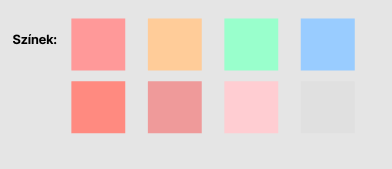
\includegraphics[width=0.45\linewidth]{images/szinek.png}}
	\hspace{5pt}
	\subcaptionbox{Gombok megjelenése}{
		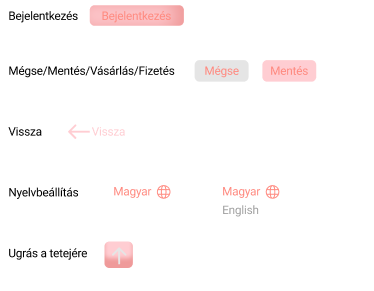
\includegraphics[width=0.45\linewidth]{images/gombok.png}}
	\caption{Figma kiegészítő elemek tervezete}
	\label{fig.picture-10}
\end{figure}

Ezeken az összefoglaló elemeken felül vázlatosan elkészítettem az egyes oldalak megjelenési tervét, amit a \ref{fig.picture-11}-es képein fellelhető. Ahogy a két képet összehasonlítjuk az alkalmazásban megjelenő oldalakkal észrevehetően nagy változásokat eszközöltem egyes megjelenéseken.
\begin{figure}[H]
	\centering
	\subcaptionbox{Bejelentkezési felület terv}{
		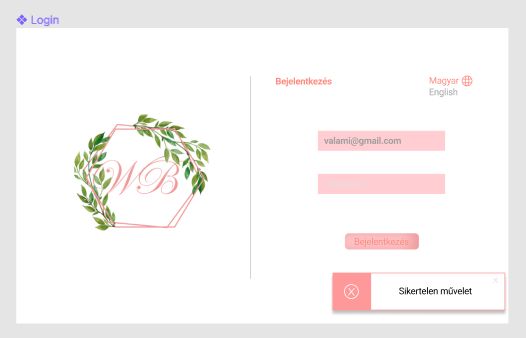
\includegraphics[width=0.45\linewidth]{images/login.png}}
	\hspace{5pt}
	\subcaptionbox{Termékek vázlatterve}{
		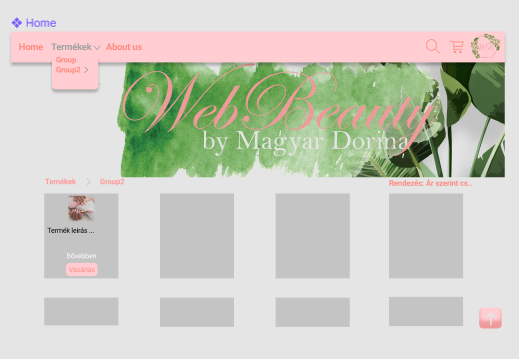
\includegraphics[width=0.45\linewidth]{images/oldal_terv.png}}
	\caption{Figma kiegészítő elemek tervezete}
	\label{fig.picture-11}
\end{figure}

\subsection{Logók és grafikai elemek}
Az alkalmazás grafikai elemei elkészítése során próbáltam figyelembe venni a program letisztult megjelenését és természetesen annak színvilágát. Az webáruházban két különböző színű logó kerül felhasználásra. A \ref{fig.picture-12}-es ábra a. képén látható sötétebb kerettel és szöveggel rendelkező logót a másik b. logón szereplő hasonló színét alkalmazó háttereken alkalmazom, mint például az oldalak menüsora. Amíg a b. logót a fehér hátterekkel rendelkező oldalakon kerül megjelenítésre.
\begin{figure}[H]
	\centering
	\subcaptionbox{Sötétebb logó}{
		
\includegraphics[width=0.45\linewidth]{images/logo_monogram_dark.png}}
	\hspace{5pt}
	\subcaptionbox{Logó}{
		
\includegraphics[width=0.45\linewidth]{images/logo_monogram.png}}
	\caption{Grafikai elemek}
	\label{fig.picture-12}
\end{figure}

A webshopon megjelenő további grafikai elemek mint például a \ref{fig.picture-13}-as ábrán található képek célja, hogy változatosabb megjelenést kölcsönözzön az alkalmazás számára.
\begin{figure}[H]
	\centering
	\subcaptionbox{Rólunk felület fejléce}{
		
\includegraphics[width=0.45\linewidth]{images/logo_name.png}}
	\hspace{5pt}
	\subcaptionbox{Főoldal felület fejléce}{
		
\includegraphics[width=0.45\linewidth]{images/logo_page_header.png}}
	\caption{Grafikai elemek}
	\label{fig.picture-13}
\end{figure}

\section{Forráskódok}

\subsection{Kliensoldali forráskódok}
Ebben az alfejezetben található a kliensoldal működésénél említett chatbot bemutatása forráskódok segítségével. Ezt a funkciót úgy került megvalósításra, hogy előre megírt és adatbázisban eltárolt kérdéseket és válaszokat kérdezek le és jelenítek meg animációk segítségével. Az alábbi forráskódok ezt tartalmazzák.

Először is lekérdezem és eltárolom ezt a chat listát a GET/chat~\ref{src:chat} forráskódban szereplő függvény  segítségével.

\lstset{caption={GET/chat lista lekérés - TypeScript}, label=src:chat}
\begin{lstlisting}[language=JavaScript]
	async ngOnInit() {
		await this.chat.getChat();
		this.chatSub = this.chat.getUpdateListener()
		.subscribe(chat => {
			this.chatList = chat;
		});
	}
\end{lstlisting}

Ezután megjelenítem ebben a listában szereplő kérdéseket HTML fájlban a \ref{src:chatHTML} forráskódban látottak szerint. Ezek a kérdések linkként szolgálnak, amik átirányítanak a kérdés animált profil oldalára ami a \ref{src:chatProfile} forráskódban látható.
\lstset{caption={Chatbot megjelenítése - HTML}, label=src:chatHTML}
\begin{lstlisting}[language=html]
	 <div class="chat-body">
		<div class="chat-link" *ngFor="let chat of chatList">
		<div (click)="loadChatProfile(chat.id)">{{chat.title}}</div>
	</div>
\end{lstlisting}

\lstset{caption={Chatbot kérdéshez tatoró szöveg megjelenítése - HTML}, label=src:chatProfile}
\begin{lstlisting}[language=html]
	<div class="animated display-message">
		<div class="chat__message chat__message_B" style="--delay: 2s">
			<div class="chat__content">
				{{selectedChat.title}}
			</div>
		</div>
		<div class="chat__message chat__message_A" style="--delay: 6s">
			<div class="chat__content">
				{{selectedChat.description}}
			</div>
		</div>
		...
\end{lstlisting}

A beszélgetés imitálásához scss-ben írt stílus fájlt használtam az alábbi \ref{src:scss} forráskódban leírtak alapján.

\lstset{caption={Chatbot beszélgetés animáció - scss}, label=src:scss}
\begin{lstlisting}
.chat__message {
	...
	transform-origin: 0 100%;
	padding-top: 0;
	transform: scale(0);
	...
	animation: message 0.15s ease-out 0s forwards;
	animation-delay: var(--delay);
	--bgcolor: var(--info-color);
	--radius: 8px 8px 8px 0;
}

.chat__message_B{
	color: var(--light-color);
	flex-direction: row-reverse;
	text-align: right;
	align-self: flex-end;
	transform-origin: 100% 100%;
	--bgcolor: var(--main-color);
	--radius: 8px 8px 0 8px;
}

.chat__message::before {
	content: "";
	flex: 0 0 40px;
	aspect-ratio: 1/1;
	background: var(--bgcolor);
	border-radius: 50%;
}
\end{lstlisting}

\subsection{Szerveroldali forráskódok}
Alább található forráskódok a 3.5.1-es fejezetben már (POST request segítségével) kifejtett JavaScriptben írt kérés mellett a többi példa lekérés látható. A programban használt végpontok, amik bemutatásra kerülnek a következők: GET, DELETE és PUT műveletek.

GET/news~\ref{src:get} végpont és a visszaérkező json fájl \ref{src:getJson}:

\lstset{caption={GET/news végpont}, label=src:get}
\begin{lstlisting}[language=JavaScript]
exports.getChat = (req, res, next) => {
	Chat.find().then(result => {
		res.status(200).json({
			message: "Chat fetched successfully",
			chat: result,
		});
	});
}
\end{lstlisting}

\lstset{caption={GET/news JSON}, label=src:getJson}
\begin{lstlisting}[language={JSON}]
{
	"message": "News fetched successfully!",
	"news": [
	{
		"_id": "61b61edfb415f9f7cc07e7a8",
		"title": "Oldal letrehozasa",
		"description": "Az oldal letrehozasa Magyar Dorina Szakdolgozata elkeszitese celjabol tortent. Jelenleg ez az oldal nem uzemel! Nem kerulnek ertekesitesre azok a termekek, amik az aruhazban talalhatoak! Ha tovabbi kerdese lenne a Rolunk feliratu menun keresztul kapcsolatba lephet velem es minden kerdesre email formajaban valaszolok. Megerteseteket elore is koszonom!",
		"imagePath": "http://localhost:3000/images/news/oldal-letrehozasa-1639325407045.png",
		"startDate": "2021-08-31T22:00:00.000Z",
		"endDate": "2021-12-14T23:00:00.000Z",
		"__v": 0
	}, ...
	]
}
\end{lstlisting}

PUT/news~\ref{src:put} végpont és a visszaérkező json fájl \ref{src:putJson}:

\lstset{caption={PUT/news végpont}, label=src:put}
\begin{lstlisting}[language=JavaScript]
exports.putNews = (req, res, next) => {
	let imagePath = req.body.imagePath;
	if(req.file) {
		const url = req.protocol + "://" + req.get("host");
		imagePath = url + "/images/news/" + req.file.filename
	}
	const news = new News({
		_id: req.body.id,
		title: req.body.title,
		description: req.body.description,
		imagePath: imagePath,
		startDate: req.body.startDate,
		endDate: req.body.endDate,
	});
	News.updateOne({_id: req.params.id}, news).then(result => {
		res.status(200).json(
		{message: "Update succsessful!"}
		);
	});
}
\end{lstlisting}

\lstset{caption={PUT/news JSON}, label=src:putJson}
\begin{lstlisting}[language={JSON}]
{
	"message": "Update succsessful!",
	"news": [
	{
		"_id": "61b61edfb415f9f7cc07e7a8",
		"title": "Oldal letrehozasa valtozas",
		"description": "Az oldal letrehozasa Magyar Dorina Szakdolgozata elkeszitese celjabol tortent. Jelenleg ez az oldal nem uzemel! Nem kerulnek ertekesitesre azok a termekek, amik az aruhazban talalhatoak! Ha tovabbi kerdese lenne a Rolunk feliratu menun keresztul kapcsolatba lephet velem es minden kerdesre email formajaban valaszolok. Megerteseteket elore is koszonom!",
		"imagePath": "http://localhost:3000/images/news/oldal-letrehozasa-1639325407045.png",
		"startDate": "2021-08-31T22:00:00.000Z",
		"endDate": "2021-12-14T23:00:00.000Z",
		"__v": 0
	}]
}
\end{lstlisting}

DELETE/news~\ref{src:delete} végpont:

\lstset{caption={DELETE/news végpont}, label=src:delete}
\begin{lstlisting}[language=JavaScript]
	exports.deleteNews = (req, res, next) => {
		News.deleteOne({_id: req.params.id}).then( result => {
			res.status(200).json({
				message: "News deleted!"
			});
		});
	}
\end{lstlisting}

\section{Tesztesetek}

\subsection{Kliensoldal tesztelése}
TBA


\subsection{Szerveroldal tesztelése}
Szerveroldal REST API kérések tesztelése Postman program segítségével. A táblázat első oszlopában a requestekre vonatkozó hitelesítési kötelezettségéről található információ. A második oszlopban a kérések URL címe olvasható, ezzel a címmel érhető el a back-end-en megírt request függvények.  A harmadik és negyedik oszlopban pedig a kérés végrehajtásáról nyújt információkat. Ilyen információ például az, hogy sikeres volt-e a művelet és milyen üzenet társul hozzá.

\begin{table}[H]
	\begin{tabular}{ | c | l | c | l | }
		\hline
		\multicolumn{4}{|c|}{\textbf{Szerveroldali végpontok tesztelése}}
		\\ \hline
		\hline
		\multicolumn{4}{|c|}{\textbf{GET}} \\
		\hline
		\multicolumn{1}{| c |}{\textbf{ Token }} & \multicolumn{1}{ c |}{\textbf{Request URL}} & \multicolumn{1}{ c | }{\textbf{Status}} & \multicolumn{1}{ c | }{\textbf{Message}} \\
		\hline		
		nem & api/products & 200 OK & Products fetched successfully  \\
		\hline
		nem & api/productsGroups &200 OK & Group fetched successfully \\
		\hline
		nem & api/news & 200 OK & News fetched successfully \\
		\hline
		nem & api/chat & 200 OK & Chat fetched successfully  \\
		\hline 
		nem & api/messages & 401 Unauthorized & Auth failed  \\
		\hline 
		igen & api/messages & 200 OK & Message fetches successfully  \\
		\hline
		igen & api/orders & TBA & TBA \\
		\hline
		\multicolumn{4}{|c|}{\textbf{POST}} \\
		\hline
		\multicolumn{1}{| c |}{\textbf{ Token }} & \multicolumn{1}{| c |}{\textbf{Request URL}} & \multicolumn{1}{ c | }{\textbf{Status}} & \multicolumn{1}{ c | }{\textbf{Message}} \\
		\hline
		igen & api/products & 500 Server Error & Unexpected field \\
		\hline
		igen & api/news & TBA & TBA \\
		\hline
		nem & api/messages & TBA & TBA \\
		\hline
		nem & api/orders & TBA & TBA \\
		\hline
		\multicolumn{4}{|c|}{\textbf{PUT}} \\
		\hline
		\multicolumn{1}{| c |}{\textbf{ Token }} & \multicolumn{1}{| c |}{\textbf{Request URL}} & \multicolumn{1}{ c | }{\textbf{Status}} & \multicolumn{1}{ c | }{\textbf{Message}} \\
		\hline
		igen & api/products & 500 Server Error & Unexpected field \\
		\hline
		igen & api/news & TBA & TBA \\
		\hline
		\multicolumn{4}{|c|}{\textbf{DELETE}} \\
		\hline
		\multicolumn{1}{| c |}{\textbf{ Token }} & \multicolumn{1}{| c |}{\textbf{Request URL}} & \multicolumn{1}{ c | }{\textbf{Status}} & \multicolumn{1}{ c | }{\textbf{Message}} \\
		\hline
		igen & api/products/6186.. & 200 OK & Products deleted \\
		\hline
		igen & api/news/61ae.. & 200 OK & News deleted \\
		\hline
		igen & api/messages/61a4.. & 200 OK & Message deleted \\
		\hline
		igen & api/orders & TBA & TBA \\
		\hline
		
	\end{tabular}
	\caption[Szerveroldali végpontok tesztelése]{Back-end REST API kérés végpontok tesztelése.}
	\label{tab:example-4}
\end{table}


\section{Továbbfejlesztési lehetőségek}